\chapter{AI: Agents}\label{AI: Agents}

\begin{figure}[H]
    \centering
    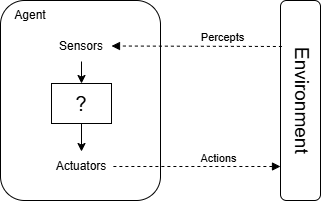
\includegraphics[
        width=0.5\linewidth, 
        height=4cm, 
        keepaspectratio
    ]{images/artificial-intelligence/ai-agents/agent-skeleton.drawio.png}
    \caption*{Agents interact with environments through sensors and actuators. \cite{common/online/tools/draw.io}}
\end{figure}


\begin{enumerate}[itemsep=0.2cm]
    \item \textbf{Agent}: An agent is anything that can be viewed as perceiving its environment through sensors and acting upon that environment through actuators.
    \hfill \cite{ai/book/Artificial-Intelligence-A-Modern-Approach/Russell-Norvig}

    \item \textbf{Rational Agent}: A rational agent is one that does the right thing
    \hfill \cite{ai/book/Artificial-Intelligence-A-Modern-Approach/Russell-Norvig}
    

    \item \textbf{Environment}: environment refers to everything outside the agent that it interacts with.
    \hfill \cite{common/online/chatgpt}

    \item \textbf{Sensors}: A sensor is any mechanism that allows an AI agent to perceive its environment by gathering information. This can be physical (hardware) or virtual (software).
    \hfill \cite{common/online/chatgpt}

    \item \textbf{Actuators}: An actuator is any mechanism that allows an AI agent to affect or change its environment by performing actions.
    \hfill \cite{common/online/chatgpt}

    \item \textbf{Percept}: agent’s perceptual inputs at any given instant
    \hfill \cite{ai/book/Artificial-Intelligence-A-Modern-Approach/Russell-Norvig}
    
    \item \textbf{Percept Sequence}: it is the complete history of everything the agent has ever perceived. In general, an agent’s choice of action at any given instant can depend on the entire percept sequence observed to date, but \textbf{not} on anything it hasn’t perceived.
    \hfill \cite{ai/book/Artificial-Intelligence-A-Modern-Approach/Russell-Norvig}

    \item \textbf{Agent Function}: maps any given percept sequence to an action; describes agent’s behavior; an external characterization of the agent; The agent function is an abstract mathematical description
    \hfill \cite{ai/book/Artificial-Intelligence-A-Modern-Approach/Russell-Norvig}

    \item \textbf{Agent Program}: internal implementation of the agent function for an artificial agent; the agent program is a concrete implementation, running within some physical system.
    \hfill \cite{ai/book/Artificial-Intelligence-A-Modern-Approach/Russell-Norvig}
\end{enumerate}

